\documentclass{article}
\usepackage{amsmath}
\usepackage{amssymb}
\usepackage{graphicx}
\usepackage{listings}
\usepackage{xcolor}
\usepackage[utf8]{inputenc}
\usepackage{titlesec}
\usepackage{mathbbol}
\usepackage{amsthm}
\usepackage{stmaryrd}


\definecolor{dkgreen}{rgb}{0,0.6,0}
\definecolor{gray}{rgb}{0.5,0.5,0.5}
\definecolor{mauve}{rgb}{0.58,0,0.82}

\lstset{frame=tb,
	language=Python,
	aboveskip=2mm,
	belowskip=5mm,
	showstringspaces=false,
	columns=flexible,
	basicstyle={\small\ttfamily},
	numbers=none,
	numberstyle=\tiny\color{gray},
	keywordstyle=\color{blue},
	commentstyle=\color{dkgreen},
	stringstyle=\color{mauve},
	breaklines=true,
	breakatwhitespace=true,
	tabsize=2
}

\begin{document}
	
	\section*{Türme von Hanoi}

	\textmd{
	Das Spiel TÜRME VON HANOI besteht aus drei Holzstäben A, B und C. Auf Stab A sind n Scheiben
	mit nach oben sukzessiv kleiner werdenden Radien aufgestapelt. Es soll ein Algorithmus gefunden
	werden, der den Turm von Stab A auf den Stab C versetzt. Dabei darf in jedem Schritt immer nur
	eine Scheibe auf einen leeren Stab oder auf eine größere Scheibe versetzt werden.
	} 
	
	\begin{figure} [h]
		\centering
		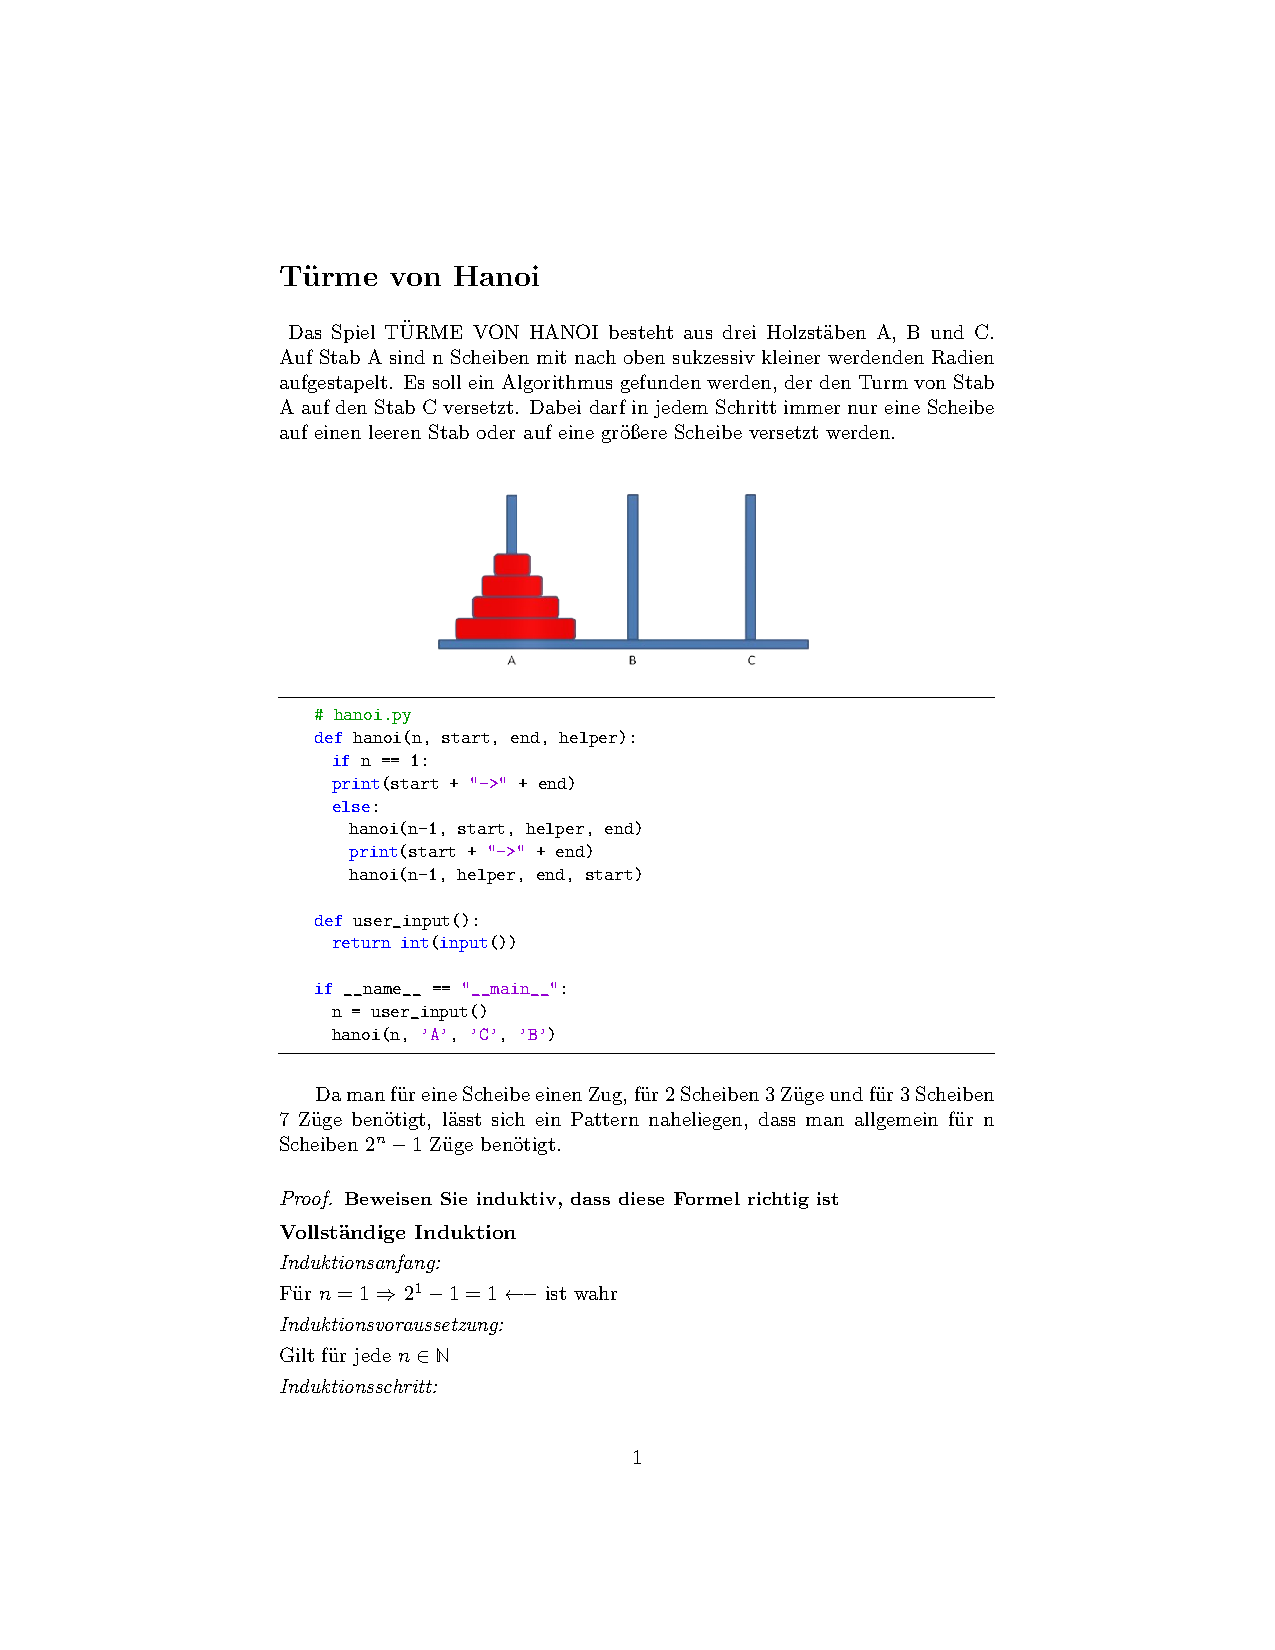
\includegraphics[width=12cm, height=4cm]{//home/thienlao/Pictures/Screenshots/hanoi.png}
	\end{figure}
	\vspace{-20pt}
	\begin{lstlisting}
		# hanoi.py
		def hanoi(n, start, end, helper): 
			if n == 1:
			print(start + "->" + end)  
			else:
				hanoi(n-1, start, helper, end)
				print(start + "->" + end)
				hanoi(n-1, helper, end, start)
		
		def user_input():
			return int(input())
		
		if __name__ == "__main__": 
			n = user_input()
			hanoi(n, 'A', 'C', 'B') 
	\end{lstlisting}
	
	\textmd{ 
	Da man für eine Scheibe einen Zug, für 2 Scheiben 3 Züge und für 3 Scheiben 7 Züge benötigt, 
	lässt sich ein Pattern naheliegen, dass man allgemein für n Scheiben $2^n - 1$ Züge benötigt. 
	} 
	
	\begin{proof}
		\section*{\small Beweisen Sie induktiv, dass diese Formel richtig ist} 
		\vspace{-2mm}
		\textbf{Vollständige Induktion} \\
		[1mm]
		\textit{Induktionsanfang:} \\
		[1mm]
		Für \( n = 1 \) $\Rightarrow$  \( 2^1 - 1 = 1 \) $\longleftarrow$ ist wahr \\
		[1mm]
		\textit{Induktionsvoraussetzung:} \\
		[1mm]
		Gilt für jede \( n \in \mathbb{N} \) \\
		[1mm]
		\textit{Induktionsschritt:} \\
		[1mm]
		Für \( n = n + 1 \) $\Rightarrow$ \( 2^{n + 1} - 1 = 2 * 2^n - 1 = 2*(2^n - 1) \) $\longleftarrow$ Voraussetzung \\
	\end{proof}
	
		\section*{\small Es ist nicht möglich, den Turm mit weniger Zügen zu versetzen}
		\vspace{-2mm}
	\textit{Annahme:} Es ist möglich, den Turm von Hanoi mit weniger als \( 2^n - 1 \) Zügen zu versetzen.  
	 	\vspace{-5pt}
		\[
		n = 1 \quad \Rightarrow \quad 2^{n-1} - 1 = 2^{1-1} - 1 = 2^0 - 1 = 0.
		\]
		Da aber mindestens 1 Zug benötigt wird, folgt, $ \lightning $
	
		\section*{Die Fibonacci-Folge}
		
		Die Fibonachi-Folge wird rekursiv definiert
		\[
		a_n = 
		\begin{cases} 
			1, & \text{für} n = 1 \\
			1, & \text{für } n = 2 \\
			a_{n-1} + a_{n-2}, & \text{für} n > 2
		\end{cases}
		\]
\end{document}